% =============================================================================
% Kapitel 4: Analyse des bestehenden Systems
% =============================================================================

Dieses Kapitel bewertet den bestehenden Prototyp von Loth und Konert~\cite{loth2022kompetenzeditor,loth2022masterprojekt} systematisch, um die Ausgangslage für die Weiterentwicklung zu bestimmen.
Die Bewertung orientiert sich am Rahmenwerk von Sommerville~\cite{sommerville2016software} für Legacy-Systeme, das für produktionsreife Software konzipiert ist und hier analog auf einen Forschungsprototyp angewandt wird, um dessen Weiterentwicklungspotenzial systematisch einzuschätzen.
Ergänzend wird ein IST-SOLL-Abgleich gegen die in Kap.~\ref{sec:methodik} definierten Anforderungen durchgeführt.

\subsection{Technische Bewertung}\label{sec:technische-bewertung}

Die technische Bewertung folgt den Bewertungsfaktoren nach Sommerville~\cite{sommerville2016software}, Kap.~9.
Dabei werden zunächst die Umgebungsfaktoren (Figure~9.10) und anschließend die Anwendungsfaktoren (Figure~9.11) betrachtet.

\paragraph{Umgebungsbewertung.}

Das gravierendste Problem des Prototyps liegt in der \emph{Supplier Stability}.
Alle drei zentralen Abhängigkeiten -- Vue~2, Nuxt~2 und Vuetify~2 -- befinden sich am Ende ihres Lebenszyklus.
Vue~2 ist seit Dezember 2023 End-of-Life~\cite{eol2026vue}, Nuxt~2 erhält seit Juni 2024 keinen Maintenance-Support mehr~\cite{eol2026nuxt} und Vuetify~2 wurde durch Vuetify~4.0.6 abgelöst~\cite{eol2026vuetify}.
Keines der drei Frameworks erhält noch Security-Patches.
Abb.~\ref{fig:nuxt-eol} veranschaulicht den Release-Zyklus von Nuxt: Zum Zeitpunkt der Entwicklung des Prototyps (2022) befand sich Nuxt~2 in aktiver Entwicklung; inzwischen ist auch die Maintenance-Phase abgeschlossen.

\begin{figure}[t!]
\caption{Release-Zyklus der Nuxt-Versionen. Der Prototyp wurde während der aktiven Entwicklungsphase von Nuxt~2 erstellt (2022). Zum Zeitpunkt dieser Arbeit (2026) ist Nuxt~4 die aktuelle Version. Datenquelle:~\cite{eol2026nuxt}.\label{fig:nuxt-eol}}
\centering
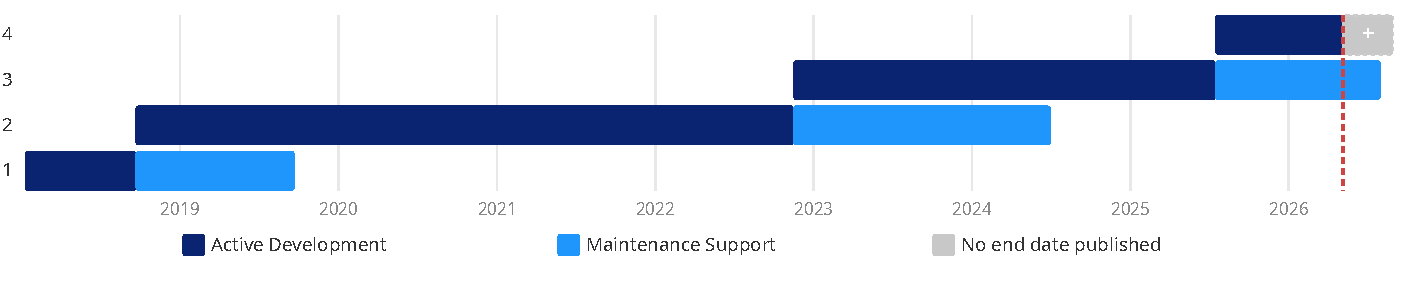
\includegraphics[width=\textwidth]{figures/nuxtoutdated.pdf}
\end{figure}

Eng damit verbunden ist die \emph{Failure Rate}: Das spaCy-Backend fehlt vollständig im Repository.
Die Prototyp-UI ist zwar lauffähig, erfordert jedoch einen manuellen Downgrade von Nuxt~3 auf Nuxt~2 sowie das separate Starten eines Docker-Containers für spaCy.
Das System ist nicht out-of-the-box reproduzierbar.

Hinsichtlich des \emph{Alters} ist der Prototyp differenziert zu bewerten.
Er wurde 2022 entwickelt, und der verwendete Stack war zum Zeitpunkt der Entwicklung aktuell -- Nuxt~2 befand sich bis November 2022 in aktiver Entwicklung~\cite{eol2026nuxt}.
Der Stack ist jedoch inzwischen veraltet, wie Abb.~\ref{fig:nuxt-eol} zeigt.

Die \emph{Performance} stellt kein Problem dar.
Die regelbasierte Analyse läuft clientseitig und verarbeitet Eingaben ohne wahrnehmbare Verzögerung; die spaCy-Tokenisierung benötigt für einzelne Sätze ebenfalls nur wenige Millisekunden.

Die \emph{Support Requirements} und \emph{Maintenance Costs} sind hingegen hoch.
Die Paketkonfiguration referenziert Nuxt~3, obwohl der Code Nuxt-2-APIs verwendet -- eine Inkonsistenz, die den Einstieg erschwert.
Das spaCy-Backend ist weder dokumentiert noch im Repository enthalten, es gibt weder CI/CD noch automatisierte Tests.
Die Abhängigkeiten können nicht aktualisiert werden, ohne Breaking Changes auszulösen, und eine inkrementelle Migration von Vue~2 auf Vue~3 ist aufgrund der fundamentalen API-Änderungen (Options API zu Composition API) nicht praktikabel.

Die \emph{Interoperability} ist neutral: Der Prototyp ist ein reiner Browser-Client ohne externe API; das spaCy-Backend stellt die einzige interne Schnittstelle dar.

\paragraph{Anwendungsbewertung.}

Die folgenden Befunde sind im Kontext eines Forschungsprototyps zu lesen, der als Proof-of-Concept konzipiert wurde und nicht den Anspruch produktionsreifer Software erhebt~\cite{loth2022masterprojekt}.

Die \emph{Understandability} der Codebasis ist eingeschränkt.
Zwar ist der Umfang mit wenigen Dateien überschaubar, doch die Hauptkomponente umfasst 1334~Zeilen und vermischt UI-Logik, NLP-Aufrufe, Verb-Matching, Scoring und Persistenz in einer einzigen Datei.
Variablennamen mischen Deutsch und Englisch; es finden sich Tippfehler in Bezeichnern und toter Code in Form leerer Methoden mit Alert-Aufrufen.

Die \emph{Documentation} beschränkt sich auf das DELFI-Paper~\cite{loth2022kompetenzeditor} und den zugehörigen Projektbericht~\cite{loth2022masterprojekt}.
Code-Dokumentation, Setup-Anleitung und API-Dokumentation für das spaCy-Backend fehlen vollständig.

Das \emph{Datenmodell} ist informell.
Das IndexedDB-Schema wird über Dexie implizit durch Seed-Daten in \texttt{db.js} definiert; alle Verblisten und Beispieltexte sind dort hardcodiert.
Die Verbliste enthält einen fehlerhaften Eintrag (\emph{Zusammenhänge} als Verb, obwohl es ein Nomen ist) sowie das Verb \emph{erkennen} in drei Taxonomiestufen ohne Disambiguierungslogik.

\emph{Performance} und \emph{Programmiersprache} sind unkritisch: JavaScript ist als Sprache aktuell und weit verbreitet; das Problem liegt nicht in der Sprache selbst, sondern in den veralteten Frameworks.

Das \emph{Configuration Management} weist die bereits genannte Inkonsistenz zwischen \texttt{package.json} und tatsächlich verwendeten APIs auf.
Es gibt kein CI/CD und keine Build-Pipeline.

Besonders gravierend ist das vollständige Fehlen von \emph{Test Data}: Es existieren keine automatisierten Tests, kein Test-Verzeichnis und kein Test-Framework in den Abhängigkeiten.

Der Original-Entwickler ist nicht am Projekt beteiligt; die Einarbeitung erfolgte durch Codeanalyse und die vorhandene Dokumentation.

\subsection{Funktionale Bewertung}\label{sec:funktionale-bewertung}

Der IST-SOLL-Abgleich stellt den aktuellen Zustand des Prototyps den definierten funktionalen und nicht-funktionalen Anforderungen gegenüber.
Tab.~\ref{tab:ist-soll} gibt eine kompakte Übersicht; die wesentlichen Befunde werden im Folgenden erläutert.

\begin{table}[H]
\caption{IST-SOLL-Abgleich: Erfüllungsstatus der Anforderungen\label{tab:ist-soll}}
\centering
\small
\begin{tabular}{llll}
\hline
\textbf{ID} & \textbf{Anforderung} & \textbf{Typ} & \textbf{Status} \\
\hline
FA1 & Klassifikation         & funktional       & teilweise erfüllt \\
FA2 & Taxonomie-Zuordnung    & funktional       & teilweise erfüllt \\
FA3 & Empfehlungen           & funktional       & teilweise erfüllt \\
FA4 & Set-Analyse            & funktional       & nicht erfüllt \\
FA5 & Echtzeit-Feedback      & funktional       & erfüllt \\
FA6 & Persistenz             & funktional       & teilweise erfüllt \\
\hline
NFA1 & Konfidenzmaße         & nicht-funktional & nicht erfüllt \\
NFA2 & Transparenz           & nicht-funktional & erfüllt \\
NFA3 & Deutsche Sprache      & nicht-funktional & erfüllt \\
NFA4 & Technologie-Migration & nicht-funktional & nicht erfüllt \\
NFA5 & Performance           & nicht-funktional & erfüllt \\
\hline
\end{tabular}
\end{table}

\paragraph{Erfüllte Anforderungen.}

Vier Anforderungen sind vollständig erfüllt und bilden die bewährten Stärken des Prototyps, die bei der Weiterentwicklung erhalten bleiben.
Das \emph{Echtzeit-Feedback} (FA5) funktioniert zuverlässig: Nach einer Tipp-Pause von 1000\,ms werden Verben farblich hervorgehoben -- grün für empfohlene, rot für nicht empfohlene, blau für NLP-erkannte und grau für nicht zugeordnete Verben.
Die \emph{Transparenz} (NFA2) ist eine besondere Stärke des regelbasierten Ansatzes: Jede Zuordnung ist direkt nachvollziehbar, da sie auf der Zugehörigkeit eines Verbs zu einer expliziten Liste basiert.
Info-Popups erklären die Bewertungslogik.
Die Unterstützung der \emph{deutschen Sprache} (NFA3) ist durch die deutsche Verbliste und das spaCy-Modell \texttt{de\_core\_news\_sm} gegeben.
Die \emph{Performance} (NFA5) ist durch die clientseitige Verarbeitung kleiner Datenmengen kein Problem.

\paragraph{Teilweise erfüllte Anforderungen.}

Die vier teilweise erfüllten Anforderungen bilden den Kern der vorliegenden Untersuchung.
In jedem Fall existiert ein funktionales Konzept im Prototyp, dessen Wirksamkeit jedoch durch die geschlossene Verbliste und die fehlende Nutzung der Taxonomie-Zuordnung begrenzt ist.

Bei der \emph{Klassifikation} (FA1) verfolgt der Prototyp einen impliziten Ansatz: Sätze ohne gelistetes Verb werden als \glqq entbehrlich\grqq\ markiert, was einer Nicht-Kompetenz-Klassifikation entspricht.
Dieses Konzept scheitert jedoch an Kompetenzformulierungen, die Verben verwenden, die nicht in der statischen Liste enthalten sind -- diese werden fälschlich als entbehrlich eingestuft.

Die \emph{Taxonomie-Zuordnung} (FA2) ist im Datenmodell angelegt: Die Verbliste in \texttt{db.js} enthält 80~Verben mit Zuordnung zu den sechs Stufen nach Anderson und Krathwohl~\cite{anderson2001taxonomy}.
Die Taxonomiestufe wird jedoch im UI nicht angezeigt; der Score ist rein binär (empfohlen/nicht empfohlen).
Darüber hinaus erscheint das Verb \emph{erkennen} in drei verschiedenen Stufen ohne Disambiguierungslogik.

Die \emph{Empfehlungsfunktion} (FA3) zeigt bei nicht empfohlenen Verben eine statische Tabelle aller empfohlenen Verben an -- immer dieselbe Liste, unabhängig vom Kontext des Satzes.
Eine ähnlichkeitsbasierte Auswahl findet nicht statt.

Die \emph{Persistenz} (FA6) unterstützt Speichern, Laden und Löschen über IndexedDB.
Die Speicherfunktion (\texttt{saveComp()}) verwendet jedoch ausschließlich \texttt{add()}, sodass jeder Speichervorgang einen neuen Eintrag erstellt, anstatt den bestehenden zu aktualisieren.

\paragraph{Nicht erfüllte Anforderungen.}

Drei Anforderungen sind nicht erfüllt.
Die \emph{Set-Analyse} (FA4) fehlt vollständig: Der Prototyp analysiert jeden Satz einzeln; es gibt keine Aggregation auf Modulebene, keine Taxonomie-Verteilung und keine Abdeckungsanalyse.
\emph{Konfidenzmaße} (NFA1) existieren nicht -- der vorhandene Score ist ein Gesamt-Qualitätsprozentsatz für den gesamten Text, kein Konfidenzwert pro Zuordnung.
Die \emph{Technologie-Migration} (NFA4) steht aus: Der gesamte Stack (Nuxt~2, Vue~2, Vuetify~2) ist End-of-Life.

\paragraph{Selbstidentifizierte Limitationen.}

Loth und Konert benennen in ihrem Fazit selbst Erweiterungswünsche, die den hier identifizierten Lücken entsprechen~\cite{loth2022kompetenzeditor,loth2022masterprojekt}.
Die Autoren fordern, dass \glqq Schlüsselwörter auch in abgewandelter, konjugierter und weiterer abweichender Form von der Software analysiert werden können\grqq~\cite{loth2022kompetenzeditor} -- eine Fähigkeit, die ein Embedding-basierter Ansatz prinzipbedingt mitbringt, da er nicht auf exakte Zeichenketten, sondern auf semantische Ähnlichkeit operiert.
Darüber hinaus identifizieren die Autoren die Möglichkeit, Texte \glqq in eine weitere Datenbank gespeist werden und mit anderen Kompetenzen dieser Domäne verglichen oder automatisch um Vorschläge aus anderen Texten ergänzt werden\grqq~\cite{loth2022kompetenzeditor} zu lassen -- dies entspricht der ähnlichkeitsbasierten Empfehlungsfunktion (FA3).
Schließlich weisen die Autoren auf die fehlende formale Evaluation hin, die durch den in dieser Arbeit erstellten Gold-Standard-Datensatz adressiert wird.

\subsection{Strategische Einordnung}\label{sec:strategische-einordnung}

Sommerville~\cite{sommerville2016software} unterscheidet vier strategische Optionen für den Umgang mit Legacy-Systemen, basierend auf einer kombinierten Bewertung von Geschäftswert und technischer Qualität:
Abschalten (\emph{Scrap}), Weiterbetreiben (\emph{Maintain}), Modernisieren (\emph{Reengineer}) oder Ersetzen (\emph{Replace}).

Der Prototyp weist einen \textbf{hohen konzeptionellen Wert} auf: Das Konzept wurde publiziert~\cite{loth2022kompetenzeditor}, die regelbasierte Analyse funktioniert zuverlässig für gelistete Verben, und vier der elf Anforderungen sind bereits erfüllt (vgl. Tab.~\ref{tab:ist-soll}).
Gleichzeitig ist die \textbf{technische Qualität niedrig}: Der Stack ist veraltet, es gibt keine automatisierten Tests, die Code-Dokumentation fehlt und die fehlende Trennung von Verantwortlichkeiten erschwert gezielte Änderungen.

Diese Kombination -- hoher Geschäftswert bei niedriger technischer Qualität -- entspricht in Sommervilles Bewertungsmatrix (Figure~9.9) dem Cluster \emph{Low quality, high business value}, für das Reengineering empfohlen wird~\cite{sommerville2016software}.
Ein Abschalten scheidet aufgrund des bewährten Konzepts aus; ein bloßes Weiterbetreiben ist nicht möglich, da die Abhängigkeiten keine Security-Patches mehr erhalten; eine vollständige Neuentwicklung wäre unverhältnismäßig, da Architektur und UI-Konzepte wiederverwendbar sind.

Die Weiterentwicklung lässt sich als Kombination zweier Wartungstypen einordnen:
\emph{Environmental Adaptation} -- die Migration des Frameworks von Nuxt~2 auf Nuxt~4 und von Vue~2 auf Vue~3 -- sowie \emph{Functionality Addition} -- die Integration der Embedding-basierten Analysefunktionen.
Dabei wird die Architektur des Prototyps beibehalten, der Quellcode jedoch aufgrund der umfangreichen Breaking Changes zwischen den Framework-Versionen weitgehend überarbeitet.
